\section*{Appendix}

\section{\LB Event Types}
\label{a:events}
Complete list of all events' names together with their description follows.
% see events.tex.T
\input{events}

\newpage
\section{\LB Job States}
\label{a:jobstat}
Complete list of all job' states together with their description follows.
% see status.tex.T
\input{status}

\begin{figure}[h]
\centering
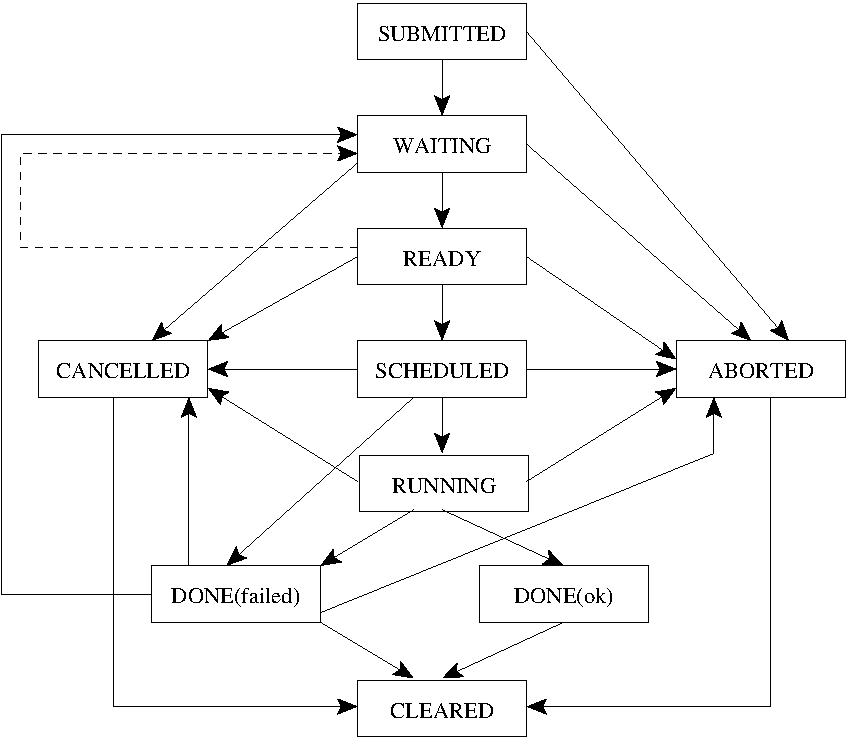
\includegraphics[width=.6\hsize]{images/wms2-jobstat}
\caption{\LB\ job state diagram}
\end{figure}

\newpage
\section{Environment variables}
\label{a:environment}

Complete list of all environment variables affecting LB behaviour follows with 
their description and default values (if applicable).

% default values can be read especially from org.glite.lb.common/src/param.c
% and apropriate header files

\begin{tabularx}{\textwidth}{l>{\raggedright\arraybackslash}X}
GLITE\_WMS\_LOG\_DESTINATION & 
   % see also glite/lb/log_proto.h (org.glite.lb.common/interface/log_proto.h)
   address of the \texttt{glite-lb-logd} daemon (for logging events), 
   in form \texttt{hostname:port},
   default value is \texttt{localhost:9002}\\
GLITE\_WMS\_LOG\_TIMEOUT & 
   % see also glite/lb/timeouts.h (org.glite.lb.common/interface/timeouts.h)
   timeout (in seconds) for asynchronous logging, 
   default value is \texttt{120} seconds, 
   maximum value is \texttt{300} seconds \\
GLITE\_WMS\_LOG\_SYNC\_TIMEOUT & 
   % see also glite/lb/timeouts.h (org.glite.lb.common/interface/timeouts.h)
   timeout (in seconds) for synchronous logging, 
   default value is \texttt{120} seconds, 
   maximum value is \texttt{600} seconds \\
GLITE\_WMS\_NOTIF\_SERVER & 
   address of the \texttt{glite-lb-bkserver} daemon (for receiving notifications)
   in form \texttt{hostname:port}, for receiving notifications,
   there is no default value,
   mandatory for \texttt{glite-lb-notify} \\
GLITE\_WMS\_NOTIF\_TIMEOUT & 
   % see also glite/lb/timeouts.h (org.glite.lb.common/interface/timeouts.h)
   timeout (in seconds) for notification registration,
   default value is \texttt{120} seconds,
   maximum value is \texttt{1800} seconds \\
GLITE\_WMS\_QUERY\_SERVER & 
   address of the \texttt{glite-lb-bkserver} daemon (for queries), 
   in form \texttt{hostname:port}, 
   there is no default value \\
GLITE\_WMS\_QUERY\_TIMEOUT &
   % see also glite/lb/timeouts.h (org.glite.lb.common/interface/timeouts.h)
   timeout (in seconds) for queries,
   default value is \texttt{120} seconds,
   maximum value is \texttt{1800} seconds \\
GLITE\_WMS\_LBPROXY\_STORE\_SOCK &
   UNIX socket location for logging to LB Proxy,
   default value is \texttt{/tmp/lb\_proxy\_store.sock} \\
GLITE\_WMS\_LBPROXY\_SERVE\_SOCK &
   UNIX socket location for queries to LB Proxy,
   default value is \texttt{/tmp/lb\_proxy\_serve.sock} \\
GLITE\_WMS\_LBPROXY\_USER &
   user credentials (DN) when communicating with LB Proxy,  
   there is no default value \\
X509\_USER\_CERT, X509\_USER\_KEY & 
   location of user credentials (certificate and private key),
   default values are \texttt{~/.globus/user{cert,key}.pem} \\
GLOBUS\_HOSTNAME & 
   hostname to appear as event origin, useful only for debugging, 
   default value is hostname \\
QUERY\_SERVER\_OVERRIDE & 
   values defined in QUERY\_SERVER will override also values in jobid in queries,
   useful for debugging only, 
   default value \texttt{no} \\
QUERY\_JOBS\_LIMIT & 
   maximal size of results for query on jobs, 
   default value is  \texttt{0} (unlimited) \\
QUERY\_EVENTS\_LIMIT & 
   maximal size of results for query on events, 
   default value is  \texttt{0} (unlimited) \\
QUERY\_RESULTS & 
   specifies behavior of query functions when size limit is reached,
   value can be \texttt{None} (no results are returned),
   \texttt{All} (all results are returned, even if over specified limit),
   \texttt{Limited} (size of results is limited to size specified by QUERY\_JOBS\_LIMIT
   or QUERY\_EVENTS\_LIMIT) \\
CONNPOOL\_SIZE & 
   maximal number of open connections in logging library,
   for developers only,
   default value is \texttt{50} \\
\end{tabularx}

For backward compatibility, all \verb'GLITE_WMS_*' variables can be prefixed by
\verb'EDG_WL_' instead, for example \verb'EDG_WL_LOG_DESTINATION'.

